% Supplementary local evidence-integration working draft: 20260930
% Frozen experiment-delivery root: 20260815-v1.0.0
\newcommand{\DoNotLoadEpstopdf}{}
\documentclass[journal]{IEEEtran}

\usepackage{booktabs}
\usepackage{graphicx}
\usepackage{amsmath,amssymb}
\usepackage{placeins}
\usepackage{cite}
\usepackage{url}

\title{Supplementary Material: Independent Content and Style Evidence for UAV--Satellite Retrieval}
\author{Chen Che}

\begin{document}
\maketitle
\markboth{Local working draft --- 30 September 2026}{Independent Content and Style Evidence}
\begin{center}\footnotesize\itshape
Local working draft: completed-result integration; remaining experiments and final review are pending.
\end{center}

\section{Completed Semantic-Model Evidence}

The official evaluation contains 42 runs and 231 run--task records. The
36 main fits produce 66 task--variant three-seed summaries over 198
run--task records. The six additional fits are seed-1 sensitivity settings
and produce 33 further task records. Tables~\ref{tab:sensitivity-r1}
and \ref{tab:sensitivity-map} retain all sensitivity results and the
matching main Full seed-1 reference for each of the 11 tasks. No SD is
assigned to a single fit. The three-seed main and transfer tables in the
main paper report sample SD with denominator $n-1=2$; they do not report
standard errors, confidence intervals, or significance decisions.

\begin{table*}[!t]
\centering
\caption{Seed-1 Full sensitivity results: R@1 (\%). The first column is the existing main Full seed-1 reference, not a three-seed mean. Each other setting uses one fit per dataset. No SD or significance is inferred. Values are rounded to three decimals; a positive value that would round to zero is shown as $<0.001$. An actual zero remains 0.000.}
\label{tab:sensitivity-r1}
\small
\setlength{\tabcolsep}{3pt}
\begin{tabular}{lrrrr}
\toprule
Task & R18/512 reference & R50/512 & R18/256 & R18/1024 \\
\midrule
University D2S & 31.906 & 35.890 & 31.771 & 32.918 \\
University S2D & 45.934 & 49.929 & 43.224 & 46.505 \\
University Street2S & 0.931 & 0.698 & 0.931 & 0.969 \\
\midrule
SUES U150$\to$S & 28.700 & 31.550 & 26.125 & 29.800 \\
SUES S$\to$U150 & 47.500 & 45.000 & 38.750 & 50.000 \\
SUES U200$\to$S & 33.150 & 36.975 & 32.125 & 34.925 \\
SUES S$\to$U200 & 61.250 & 50.000 & 46.250 & 43.750 \\
SUES U250$\to$S & 35.975 & 42.200 & 35.200 & 35.700 \\
SUES S$\to$U250 & 60.000 & 53.750 & 47.500 & 50.000 \\
SUES U300$\to$S & 38.775 & 46.675 & 36.000 & 36.200 \\
SUES S$\to$U300 & 60.000 & 57.500 & 60.000 & 55.000 \\
\bottomrule
\end{tabular}
\end{table*}

\begin{table*}[!t]
\centering
\caption{Seed-1 Full sensitivity results: official trapezoidal mAP (\%). The first column is the existing main Full seed-1 reference, not a three-seed mean. Each other setting uses one fit per dataset. No SD or significance is inferred. Values are rounded to three decimals; a positive value that would round to zero is shown as $<0.001$. An actual zero remains 0.000.}
\label{tab:sensitivity-map}
\small
\setlength{\tabcolsep}{3pt}
\begin{tabular}{lrrrr}
\toprule
Task & R18/512 reference & R50/512 & R18/256 & R18/1024 \\
\midrule
University D2S & 38.142 & 41.974 & 37.913 & 38.908 \\
University S2D & 29.240 & 34.499 & 29.009 & 30.088 \\
University Street2S & 2.185 & 1.969 & 2.335 & 2.237 \\
\midrule
SUES U150$\to$S & 37.158 & 38.837 & 34.800 & 38.430 \\
SUES S$\to$U150 & 34.282 & 32.035 & 29.901 & 32.113 \\
SUES U200$\to$S & 41.465 & 44.323 & 40.568 & 43.465 \\
SUES S$\to$U200 & 40.246 & 37.113 & 35.711 & 36.900 \\
SUES U250$\to$S & 44.434 & 49.131 & 43.424 & 44.457 \\
SUES S$\to$U250 & 43.996 & 41.645 & 38.474 & 39.406 \\
SUES U300$\to$S & 47.108 & 53.093 & 44.307 & 45.021 \\
SUES S$\to$U300 & 45.247 & 44.647 & 41.942 & 40.986 \\
\bottomrule
\end{tabular}
\end{table*}


\subsection{Corruption Metrics and Evidence Path}

The four dataset--variant seed-1 runs evaluate six query-corruption families
at five severities, yielding 660 task-level corrupted evaluations and 22
clean references. The aggregate retains six metrics per corrupted task
evaluation (3,960 rows). The R@1 and official mAP plot sources contain
1,320 of these rows, with all tasks and severities retained. Relative
retention is $100m_{\mathrm{corrupt}}/m_{\mathrm{clean}}$; the percentage-point
drop is $100(m_{\mathrm{clean}}-m_{\mathrm{corrupt}})$ for metric fractions.
Neither substitutes for the absolute corrupted metric. All supplied clean
denominators are positive; a zero denominator would make retention undefined.

Full uses cached CLIP evidence for clean evaluation and online CLIP evidence
for corrupted queries. The 64-image clean diagnostic has no numerical
equivalence threshold, so it establishes neither bitwise parity nor
negligible effects on ranking. The curves combine pixel corruption with
this evidence-path difference. They are seed-1 descriptive measurements,
with no pooling across tasks, directions, heights or severities.

\subsection{Clean-Query Diagnostic Definitions}

T4's shared Visual-margin quartiles use linear 25th, 50th and 75th percentile
cutpoints, with equality assigned to the lower interval. Full is aligned
to Visual query order before applying the same mask. Quartiles are ordered
categories rather than equal numerical margin intervals or necessarily
equal-sized groups. The 132 margin strata comprise 84 groups meeting the
registered 100-query threshold and 48 groups of 20 queries that do not.
Eligibility is a count threshold, not evidence of significance. Other
entropy and semantic strata remain outside the independently recounted
membership/value scope.

For T5, let $N$ be the full task's query count and let
$k=\lceil cN\rceil$ at requested coverage $c$. Realized coverage is $k/N$.
Each variant independently selects the leading $k$ queries after stable
descending ordering by raw Top-1-minus-Top-2 cosine margin. The selective
risk denominator is $k$; coverage-constrained success uses $N$ and counts
queries that are both selected and correct. The selected-set overlap counts
membership selected by both variants, not correctness shared by both.
At full coverage, success equals ordinary R@1.

The 66 native task--seed--variant series retain ten requested coverages
from 0.1 to 1.0 (660 stored points). Saved AURC is computed upstream over
all query prefixes, not by integrating those ten plotted points. The 132
paired records use the four requested coverages 0.5, 0.75, 0.9 and 1.0;
the 0.75 records are separate observations, not interpolation from the
native ten-point display.

The fixed reliability score is
$\operatorname{clip}((s_1-s_2)/2,0,1)$, where $s_1-s_2$ is the cosine
margin. It is not a posterior probability. All 15 bins for each of the
66 series are retained (990 bin records): 140 occupied and 850 empty.
Empty-bin count is zero while mean score and accuracy are undefined, not
zero. ECE is the saved count-weighted absolute score--accuracy gap, a
fraction rather than an accuracy percentage. A lower ECE can accompany
lower accuracy and is not by itself evidence of improved probability
calibration. Visual and Full can place different queries in the same
numbered bin.

\subsection{Statistical and Provenance Scope}

The 33-comparison family for official Visual-versus-Full results is distinct
from the T4 eligible 284-comparison family and the 132 T5 paired records.
The completed query audit independently recounted the 132 shared margin
strata and recomputed the 66 T5 native and 132 paired query records from
their stored per-query inputs. Entropy/semantic-stratum memberships and
values were not independently recomputed. T4 exact McNemar calculations
were checked from saved discordance counts, with query recount restricted
to the shared margin strata. Retained bootstrap intervals were not
independently resampled or accepted as new inferential evidence; this draft
does not use them to claim significance for the semantic results. These
limits do not redefine the separate historical public-baseline analyses.

This result integration formats existing measured summaries. Checkpoint,
cache and full image-content SHA evidence is inherited, with documented
historical metadata-chain gaps. It introduces no fresh model inference,
full-ranking reconstruction or recomputation of AP from all positive ranks.
The source tables and detailed provenance accompany this local working
draft; these limits apply to both main and supplementary semantic results.


\section{Historical Public-Baseline Query Alignment}

The analysis uses retained per-query University-1652 outputs from four fully
trained public baselines: Global CNN with Google imagery, LPN without Google
imagery, LPN, and LPN with CA-HRS.  Comparisons align query paths and location labels across methods and
retrieval rules.  This produces 37,855 drone-to-satellite (D2S) queries nested within
701 location identities and 701 satellite-to-drone (S2D) queries, one per
identity.  The analysis operates on the stored feature matrices and per-query
retrieval outputs.

\section{Numerical Results}

Tables~\ref{tab:formal-baseline-exact}--\ref{tab:formal-best-fusion} provide
the numerical values behind the separate historical public-baseline
result summaries in the main paper.
The exact baseline table uses the public per-query CUDA operation and reverse
NumPy sorting.  The paired table uses the same exact path-aligned per-query outputs for
point estimates, intervals, and tests. The controlled ranking-rule,
gallery-scale, and fusion analyses use a separate vectorized ranking
implementation; near-tie ordering can differ from exact per-query ranking.

\begin{table*}[!t]
\centering
\small
\caption{Exact local reproduction of four fully trained University-1652 baselines. Scores use the public per-query CUDA operation \texttt{gallery @ query} and the official trapezoidal mAP definition. All metrics are percentages.}
\label{tab:formal-baseline-exact}
\begin{tabular}{llrrrrr}
\toprule
Direction & Method & R@1 & R@5 & R@10 & mAP & MRR \\
\midrule
D2S & Global CNN + Google & 61.91 & 81.92 & 87.35 & 66.42 & 70.93 \\
D2S & LPN w/o Google & 76.62 & 90.37 & 93.60 & 79.72 & 82.82 \\
D2S & LPN & 76.75 & 90.54 & 93.97 & 79.88 & 83.02 \\
D2S & LPN + CA-HRS & 76.94 & 90.52 & 93.82 & 80.04 & 83.13 \\
\midrule
S2D & Global CNN + Google & 79.60 & 85.59 & 87.87 & 62.73 & 82.39 \\
S2D & LPN w/o Google & 87.02 & 90.73 & 92.58 & 76.79 & 89.01 \\
S2D & LPN & 86.73 & 91.30 & 93.30 & 76.42 & 88.97 \\
S2D & LPN + CA-HRS & 87.45 & 91.87 & 93.15 & 76.58 & 89.51 \\
\bottomrule
\end{tabular}
\end{table*}

\begin{table*}[!t]
\centering
\small
\caption{Exact query-paired R@1 comparisons against LPN+CA-HRS. Confidence intervals use 10,000 paired bootstrap samples; two-sided exact McNemar tests are Holm-corrected over all 12 directional method pairs.}
\label{tab:formal-baseline-exact-significance}
\begin{tabular}{lllrrr}
\toprule
Direction & Method A & Method B & $\Delta$R@1 & 95\% CI & $p_{\rm Holm}$ \\
\midrule
D2S & Global CNN + Google & LPN + CA-HRS & +15.03 & [+14.57, +15.49] & $<10^{-300}$ \\
D2S & LPN w/o Google & LPN + CA-HRS & +0.32 & [-0.04, +0.69] & 0.513 \\
D2S & LPN & LPN + CA-HRS & +0.19 & [-0.16, +0.53] & 1 \\
S2D & Global CNN + Google & LPN + CA-HRS & +7.85 & [+5.28, +10.41] & $2.86\times10^{-8}$ \\
S2D & LPN w/o Google & LPN + CA-HRS & +0.43 & [-1.43, +2.43] & 1 \\
S2D & LPN & LPN + CA-HRS & +0.71 & [-1.57, +3.00] & 1 \\
\bottomrule
\end{tabular}
\end{table*}

\begin{table*}[!t]
\centering
\small
\caption{Controlled retrieval rules averaged over the four fully trained baselines.}
\label{tab:formal-retrieval-rules}
\begin{tabular}{lrrrrrr}
\toprule
Retrieval rule & D$\rightarrow$S R@1 & D$\rightarrow$S mAP & D$\rightarrow$S MRR & S$\rightarrow$D R@1 & S$\rightarrow$D mAP & S$\rightarrow$D MRR \\
\midrule
Cosine & 73.06 & 76.52 & 79.98 & 85.20 & 73.13 & 87.47 \\
CSLS-k10 & 74.68 & 78.34 & 82.00 & 88.80 & 78.05 & 90.57 \\
Reciprocal-k10 & 72.77 & 76.29 & 79.82 & 85.20 & 73.14 & 87.48 \\
AQE-k10 & 73.05 & 75.68 & 78.30 & 85.20 & 81.16 & 85.81 \\
AQE+CSLS-k10 & 73.06 & 75.51 & 77.97 & 85.16 & 82.60 & 85.86 \\
\bottomrule
\end{tabular}
\end{table*}

\begin{table*}[!t]
\centering
\small
\caption{Gallery-size scaling for cosine retrieval, averaged over four formal
baselines. Every reduced gallery retains all positives and uses the same
path-hash-ordered negatives for every method.}
\label{tab:formal-gallery-scale}
\begin{tabular}{lrr@{\qquad}lrr}
\toprule
D2S gallery & R@1 & mAP & S2D gallery & R@1 & mAP \\
\midrule
100      & 88.03 & 90.01 & 1,000  & 94.76 & 94.87 \\
250      & 82.64 & 85.24 & 5,000  & 91.19 & 88.35 \\
500      & 77.96 & 81.02 & 10,000 & 89.19 & 84.42 \\
750      & 75.31 & 78.57 & 25,000 & 87.05 & 78.44 \\
951 (all)& 73.06 & 76.52 & 51,355 (all)& 85.20 & 73.13 \\
\bottomrule
\end{tabular}
\end{table*}

\begin{table*}[!t]
\centering
\small
\caption{Strongest path-aligned z-score fusion versus the strongest single
baseline (LPN+CA-HRS). Fusion combines LPN without Google, LPN, and
LPN+CA-HRS. Intervals here use 10,000 ordinary query-paired bootstrap
resamples; the main-text complementarity analysis reports the corresponding
location-cluster sensitivity analysis. Exact McNemar tests are Holm-adjusted
over the two directions.}
\label{tab:formal-best-fusion}
\begin{tabular}{lrrrrrrr}
\toprule
Direction & Single R@1 & Fusion R@1 & $\Delta$R@1 [95\% CI]
& Single mAP & Fusion mAP & $\Delta$mAP & $p_{\rm Holm}$ \\
\midrule
D2S & 76.94 & 80.85 & +3.91 [3.62, 4.19]
    & 80.04 & 83.52 & +3.48 & $2.71{\times}10^{-163}$ \\
S2D & 87.45 & 89.16 & +1.71 [0.14, 3.28]
    & 76.58 & 80.46 & +3.88 & 0.0428 \\
\bottomrule
\end{tabular}
\end{table*}


\section{Published Reference Comparisons}

Table~\ref{tab:literature_sues} lists MEAN and CDM-Net results on SUES-200 at
each flight height. The rows follow the image inputs and training settings
in their source papers. Table~\ref{tab:literature_transfer} reports the
University-1652-to-SUES-200 transfer setting from InfoGeo v5, including its
relational-distillation variant. These tables retain the published metrics
and source table identifiers.

\begin{table*}[t]
\centering
\caption{Author-reported SUES-200 results (\%) by flight height.}
\label{tab:literature_sues}
\fontsize{9}{10.5}\selectfont
\setlength{\tabcolsep}{3.3pt}
\renewcommand{\arraystretch}{1.12}
\begin{tabular}{llrrrrrrrr}
\toprule
Method & Direction & \multicolumn{2}{c}{150 m} & \multicolumn{2}{c}{200 m} & \multicolumn{2}{c}{250 m} & \multicolumn{2}{c}{300 m} \\
\cmidrule(lr){3-4}\cmidrule(lr){5-6}\cmidrule(lr){7-8}\cmidrule(lr){9-10} & & R@1 & AP & R@1 & AP & R@1 & AP & R@1 & AP \\
\midrule
MEAN \cite{mean2025} & UAV $\rightarrow$ sat. & 95.50 & 96.46 & 98.38 & 98.72 & 98.95 & 99.17 & 99.52 & 99.63 \\
MEAN \cite{mean2025} & Sat. $\rightarrow$ UAV & 97.50 & 94.75 & 100.00 & 97.09 & 100.00 & 98.28 & 100.00 & 99.21 \\
CDM-Net \cite{cdmnet2025} & UAV $\rightarrow$ sat. & 93.78 & 95.16 & 97.62 & 98.16 & 98.28 & 98.69 & 99.20 & 99.31 \\
CDM-Net \cite{cdmnet2025} & Sat. $\rightarrow$ UAV & 95.25 & 92.24 & 98.50 & 96.40 & 99.00 & 97.60 & 99.00 & 98.01 \\
\bottomrule
\end{tabular}
\par\vspace{2pt}\begin{minipage}{\textwidth}\fontsize{9}{10.5}\selectfont MEAN uses RGB images at 384 pixels; CDM-Net uses generated descriptions and synthesized views at 512 pixels. Sources: MEAN Tables III/IV and CDM-Net Table IV.\end{minipage}
\end{table*}

\begin{table*}[t]
\centering
\caption{Published University-1652-to-SUES-200 transfer results (\%).}
\label{tab:literature_transfer}
\fontsize{9}{10.5}\selectfont
\setlength{\tabcolsep}{3.3pt}
\renewcommand{\arraystretch}{1.12}
\begin{tabular}{llrrrrrrrr}
\toprule
Method & Direction & \multicolumn{2}{c}{150 m} & \multicolumn{2}{c}{200 m} & \multicolumn{2}{c}{250 m} & \multicolumn{2}{c}{300 m} \\
\cmidrule(lr){3-4}\cmidrule(lr){5-6}\cmidrule(lr){7-8}\cmidrule(lr){9-10} & & R@1 & AP & R@1 & AP & R@1 & AP & R@1 & AP \\
\midrule
InfoGeo \cite{infogeo2026} & UAV $\rightarrow$ sat. & 90.87 & 92.53 & 94.20 & 95.12 & 96.08 & 96.30 & 96.31 & 96.75 \\
InfoGeo (+RD) \cite{infogeo2026} & UAV $\rightarrow$ sat. & 91.80 & 93.18 & 95.40 & 96.15 & 96.58 & 97.08 & 96.48 & 97.00 \\
\bottomrule
\end{tabular}
\par\vspace{2pt}\begin{minipage}{\textwidth}\fontsize{9}{10.5}\selectfont Source: InfoGeo v5, Table 9. Training source: University-1652; evaluation target: SUES-200. RD denotes relational distillation. Input size is 448 pixels.\end{minipage}
\end{table*}


\section{Retrieval-Rule Sensitivity}

Each of four alternatives---CSLS-k10, Reciprocal-k10, AQE-k10, and
AQE+CSLS-k10---is compared with cosine ranking for every method and direction.
The resulting 32 paired Top-1 comparisons form one complete family.  Exact
two-sided McNemar probabilities are adjusted with the Holm procedure across
that family.  Average-precision changes are paired descriptive means; they do
not receive binary McNemar inference.

Figure~\ref{fig:supp-rule-sensitivity} shows that CSLS-k10 increases Recall@1
in all eight method--direction comparisons by 0.97--3.85 percentage points,
and all eight changes remain significant after correction.  Reciprocal-k10
reduces D2S Recall@1 by 0.18--0.39 points for all four methods; these four
reductions also remain significant.  AQE-based variants leave Top-1 outcomes
mostly unchanged while altering rank-sensitive average precision, especially
for S2D.  Each comparison holds the trained checkpoint and query set fixed.

\begin{figure*}[!t]
  \centering
  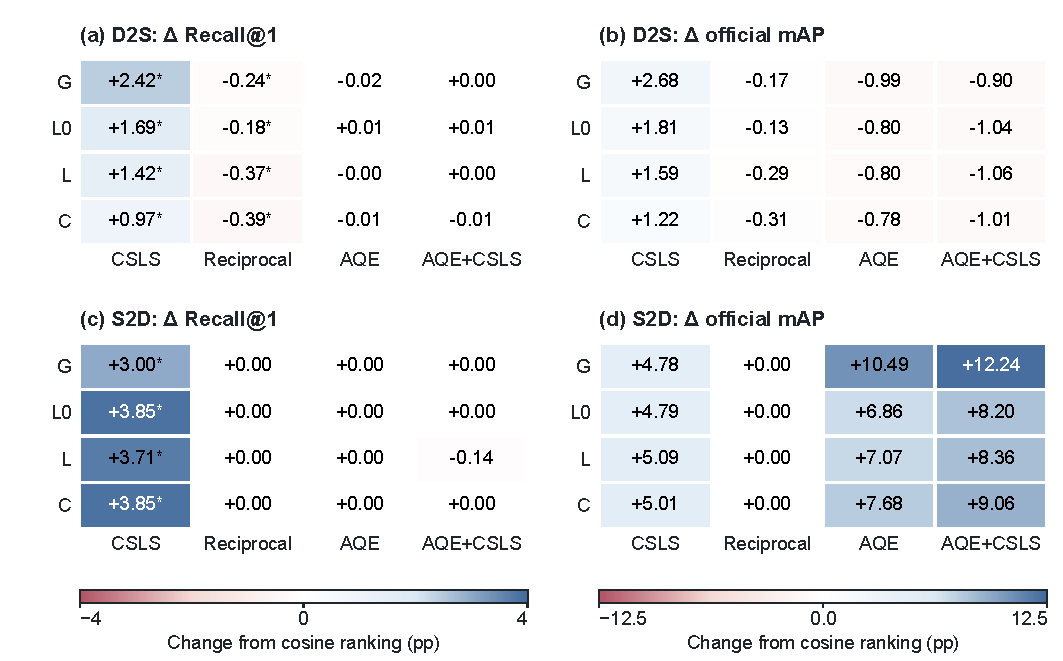
\includegraphics[width=180mm]
    {figures/journal_20260914/fig06_rule_sensitivity.pdf}
  \caption{Controlled retrieval-rule sensitivity on the same path-aligned full-gallery queries. The upper and lower rows show D2S and S2D, respectively; panels (a,c) show changes in Recall@1, and panels (b,d) show changes in official trapezoidal mAP. Values are percentage-point changes from cosine ranking, with $k=10$ for all rules. Each metric shares one zero-centered color scale across directions. Asterisks denote exact two-sided McNemar tests with Holm-adjusted $p<0.05$ across 32 comparisons; mAP changes are descriptive. G: Global CNN+Google; L0: LPN without Google; L: LPN; C: LPN+CA-HRS.}
  \label{fig:supp-rule-sensitivity}
\end{figure*}

\section{Qualitative Selection Rule}

The Top-5 image plate uses the lexicographically first path-aligned D2S query
for which LPN+CA-HRS is incorrect at rank 1 and the retained three-model
fusion is correct.  This rule is evaluated before image display.  The source
table records the query path, identity, retrieved paths, ranks, correctness,
and scores for both rows.  The aggregate rescue and harm counts summarize how frequently this
behavior occurs in the query set.

\section{Statistical Analysis and Subset Selection}

The error-complementarity oracle counts a query as correct when at least
one of the four baselines retrieves the correct identity at rank 1. It
therefore measures the observed union of their successes. The retained
fusion subset was selected on the evaluation set. Its identity-cluster
bootstrap intervals condition on that selection and measure variation
across resampled locations. The broader D2S baseline and retrieval-rule
comparisons use paired query images as inferential units. Repeated images
from the same location can be correlated, which narrows query-level
intervals relative to an analysis that retains location clusters. The
machine-readable records contain the resampling settings, comparison
families, query counts, source hashes, and software versions.

\section{Semantic Evidence Cache and Reproducibility}
\label{app:supp-provenance}

Table~\ref{tab:evidence} reports evidence-cache integrity.  Each image has one unique relative-path entry. Probability rows are
finite, nonnegative within numerical tolerance, and normalized to sum to
one.  The model revision, vocabulary
order, metadata hash, and cache hash are recorded alongside the arrays.

\begin{table*}[t]
\centering
\caption{Frozen evidence-cache integrity. Hashes show the first 10
hexadecimal characters of each SHA-256 digest.}
\label{tab:evidence}
\small
\setlength{\tabcolsep}{4pt}
\begin{tabular}{lrrr}
\toprule
Dataset & Rows & Coverage & Cache hash\\
\midrule
University-1652 & 146,520 & 100\% & 8a2333d58d\\
SUES-200        &  40,200 & 100\% & 6c3a82fdcf\\
\bottomrule
\end{tabular}
\end{table*}

Each run stores command and environment metadata, pretrained-weight records,
evidence/data/code hashes, the sampler schedule, training history, checkpoint,
and status.  Official evaluation additionally stores aggregate metrics and
per-query paths, labels, AP, reciprocal rank, margins, Top-1 correctness, and
retrieved paths.  The checkpoint record identifies its training epoch and associated
evaluation outputs.

Reproducing a comparison requires the same text order, frozen encoder,
cache arrays, and per-run configuration. These identifiers accompany the
probability inputs and retrieval checkpoints.

\section{Semantic-Model Protocol Details}

The completed main protocol comprises two datasets, six input configurations,
and three seeds, for 36 independent 80-epoch fits. Six additional seed-1 full-model fits
change ResNet-18 to ResNet-50 or the descriptor width from 512 to 256 or
1024 on each dataset. The completed matrix contains 42 fits. QDFL, FSRA, SDPL,
CCR, and MCCG define pending external visual-comparison targets; no completed
results for those comparisons are asserted in this working draft.

\subsection{Data Inventory and Training Schedule}

The University-1652 evidence inventory contains 146,520 images. The formal
protocol uses 137,576 supported official rows and excludes 8,944 auxiliary
Google-view images. The SUES-200 inventory contains all 40,200 images.
Image paths join the cached evidence to the official task manifest;
CLIP scores the pixels of each image against the fixed vocabularies.

Every official training query is scheduled at least once per epoch. A fixed
least-loaded-bin allocation gives 652 optimizer steps per University-1652
epoch and 375 per SUES-200 epoch. Training uses the official training identities and a predetermined final
epoch. A separate evaluation command applies the final checkpoint to the
official retrieval tasks.

\subsection{Statistical Implementation}

For discordant Top-1 counts $b$ and $c$, the exact two-sided McNemar
probability is
\begin{equation}
  p=\min\!\left\{1,
    2\sum_{k=0}^{\min(b,c)}\binom{b+c}{k}2^{-(b+c)}\right\}.
\end{equation}
The sum is evaluated in log space, and very small values are reported as
numerical bounds rather than zero. Holm correction is applied within the
declared comparison family. The official semantic-model protocol defines a 33-test family
across three seeds and 11 official tasks. It is distinct from the T4/T5
diagnostic records described above; the retained semantic bootstrap
intervals have not been independently resampled. The public-baseline analysis uses a 12-comparison
exact-reproduction family and a 32-comparison retrieval-rule family. Each
adjustment is applied within its full declared family.

\subsection{Experiment Records}

The experiment record links the final checkpoint to its training
configuration, software and code identifiers, logs, timing records, and
path-aligned per-query arrays. The corruption protocol links visual/full
seed-1 checkpoints to the corresponding clean-reference evaluation so that
each perturbation is measured against the same model.

\FloatBarrier
\bibliographystyle{IEEEtran}
\bibliography{refs}
\end{document}
